\documentclass[11pt]{article}
\usepackage{acl2014}
\usepackage{times}
\usepackage{url}
\usepackage{amsmath}
\usepackage{latexsym}
\usepackage{algorithm, algpseudocode, graphicx}

%\setlength\titlebox{5cm}

% You can expand the titlebox if you need extra space
% to show all the authors. Please do not make the titlebox
% smaller than 5cm (the original size); we will check this
% in the camera-ready version and ask you to change it back.


\title{Analyzing Tweets for Topic Classification}

\author{Logan Short, Vishnu Sundaresan, Christopher Wong \\
  Department of Computer Science, Stanford University \\
  {\tt \{lshort,vishnu,crwong\}@stanford.edu}}

\date{}

\begin{document}
\maketitle
\begin{abstract}
Since Twitter's introduction to social media of the hashtag as a content grouping label in 2007, the symbol and its associated usage as a classification label has seen widespread adoption throughout social media and other platforms. While the content of a post can be conveniently classified using said post's hashtags, classifying posts that do not contain hashtags proves to be a much more challenging problem. In this paper we propose a system for identifying a post's hashtags using only the non-hashtag terms of the post, and by extension address the issue of classifying the contents of posts that do not contain hashtags.
\end{abstract}

\section{Introduction}

With an overarching goal of making sense of the massive amount of Twitter data in the form of Tweets, our project focuses on characterizing Tweets by their associated specific topics, ignoring the occurrences of hashtags. In addition to simply using standalone learning models such as a bag-of-words model, neural networks on the raw frequencies, or similarity measures, we create an ensemble out of many features of a Tweet. By using the information provided by other information extraction methods such as sentiment analysis, our learning models will potentially be able to yield better results and handle more robust instances of Tweets. This project has the additional utility of being able to be integrated into other supervised learning models that require further dimensions and information about raw Tweets. The generated mapping from Tweet content to hashtag could also be used as the basis for a hashtag recommendation system for Twitter.

\section{Previous Work}

We first surveyed recent literature and research analyzing Twitter data to develop an understanding of work that has been done in the field. Sections 2.1 to 2.3 provide a brief of overview of 3 papers which significantly influenced and motivated our project. Section 2.4 outlines the new ideas and goals behind our work.

\subsection{Lee, Palsetia, Narayanan, Patwary, Agarwal, Choudhary}

The basis for Lee et. al. and its motivation is related to Twitter's Trending Topics product, which appears at the stream homepage for users. Most of the time, it is hard to classify or understand what these topics are really about, so the authors set out to classify these topics into 18 different general categories. Lee et al. [1] used two different approaches to solve this problem, including the Bag-of-Words model as well as a network-based classification. In order to come up with the labels initially used for training, they used up to 3 human annotators, with the third being used in the event that the first two did not agree on a category. Focusing on the Bag-of-Words model, the paper constructed word vectors from the trending topic definitions and related Tweets and used tf-idf weighting with a multinomial Naive Bayes classifier to classify topics that appeared. We plan on using some of these same techniques in our implementation of the topic classifier.

\subsection{Ramage, Dumais, Liebling}

Ramage et. al [2] also discuss two different features that Twitter and it's users would find useful: the process of user and figure discovery, as well as feed filtering based on one’s interests. Their work revolves around the use of a partially supervised learning model, Labeled LDA, in order to process the multi-labeled fields in Twitter data and separate it into different dimensions. The concept of labeling each document, or Tweet in this case, by a specific set of topics helps to characterize the following and reading behaviors of its users. The four main behavior classes that the paper considers are substance, status, style, and a social context to each Tweet, with data that does not fall into one of these categories being separated. Some interesting observations in specific were that certain Twitter features such as mentions, hashtagging, emoticons, replies, retweets, and favorites all were related to specific behavioral characteristics. Our project would help augment this approach by coming up with a way to label Twitter stream data, as well as potentially take away from their conclusions in our own topic classification.

\subsection{Li, Ritter, Cardie, Hovy}

The process of extracting events and classifying them based on Tweets by Li et. al. [3] can be broken down into three separate areas of work: user-level analysis, identification and extraction of public events, and learning from these areas to acquire more data. The paper proposes a pipeline by which these different areas come together to be able to classify a user’s Tweets into specific life events. Their process first takes a noisy input stream of user Tweets, and attempts to divide them up into different categories of major life events (many are not seen or captured). In order to better recognize when a major life event is captured in a Tweet, they leverage Tweet replies to determine when congratulations or condolences were being exchanged. Next, Li et al. took these different categories and trained a classifier that would use words in the Tweet, named entity tags, and the top words associated with each pre-determined category to determine which life-event (if any) it belonged to. Different signals such as the sentiment of a Tweet as described by Li et. al. can prove to be very useful, a strategy we plan on employing rather than using simply the raw text for training.

\subsection{Motivation and Goal for our Work}

Among a large number of the papers we reviewed, we found a consistent trend in that each group applied different approaches to the same problem. The majority of papers begin with a first attempt to solve the problem based purely on an information retrieval-esque language model such as n-gram likelihoods, Bag-of-Words representations, or similarity measures. These often came to the conclusion that many aspects or features in the data were being largely unused, or could not be feasibly used. The next attempts to make sense of the data involved supervised learning in the form of a neural network, or trying to uncover relationships between features using methods such as SVM. Some papers recognize the benefits of using each of these techniques, and create ensembles of different signals and successful methods in order to improve upon their accuracy.

The goal of our project is to create a simple Tweet classification system that predicts the topic of a Tweet given its text content. We aim to model Twitter data using various natural language understanding (NLU) techniques similar to those covered above and also methods discussed in CS 224U.  One of the overarching takeaways from the previous work is that ensemble systems usually yield improved performance over standalone models and learning algorithms. Previous ensemble algorithms, however, seem to use only models that are all specific to one general area of NLU, such as focusing on word representations or semantic parsing. Our system uses models based off of different areas of NLU, and in Section 5.2, we implement a new, data-driven ensemble algorithm that attempts to yield the best performance.

\section{Data Collection and Preprocessing}

We begin by discussing our data collection in Section 3.1, and in Section 3.2, we describe our methodology for cleaning and preparing the dataset of Tweets.

\subsection{Data Collection}
Twitter contains a wealth of data on an extremely diverse set of topics, and it has been often been used as a primary source of data for natural language understanding and machine learning research. Twitter, as a company, has also enabled open access to their data through company-supported APIs. As such, Twitter data is relatively easy to find and many sources of high quality Twitter data have been made available online. Our data set, provided by the Stanford Linguistic Data Consortium (LDC), contains approximately 8 gigabytes of documents containing Tweet content and metadata. The data is divided into 27 groups based on the presence of certain hashtags.\footnote{The complete list of groups (with the \# symbol removed) is: \texttt{android}, \texttt{basic}, \texttt{coffee}, \texttt{dontjudgeme}, \texttt{earthquake}, \texttt{egypt}, \texttt{election}, \texttt{freedom}, \texttt{god}, \texttt{haiti}, \texttt{happy}, \texttt{harrypotter}, \texttt{healthcare}, \texttt{immigration}, \texttt{indonesia}, \texttt{ipod}, \texttt{love}, \texttt{mubarak}, \texttt{obama}, \texttt{obamacare}, \texttt{question}, \texttt{sotu}, \texttt{teaparty}, \texttt{tsunami}, \texttt{usa}, \texttt{win}, \texttt{wiunion}.} The overall choice of groups provides a nice amount of variation in content. For our system, we used the identifying hashtag as the topic label.

Given the scope of our project and the hardware available to us, we chose to look primarily at a smaller portion of the data containing 6,000 Tweets from each of the 27 topic groups. This yields a total of 162,000 total Tweets. This smaller subset of the raw data allowed us to work more flexibly and efficiently. To verify the appropriateness of our partition size, we initially generated some of our intermediate results on larger subsets of the entire dataset. The results were sufficiently close enough to indicate that our primary working set was indeed large enough to capture the bulk of language-based variance among the Tweets. From this point on in our paper, any mention of the ``dataset'' are referencing this subset.

\subsection{Tweet Tokenization}
The vast majority of content on Twitter is generated by users, and often times, Tweets do not follow formal language conventions. As a result, it is a common occurrence for Tweets to contain words or tokens that are not normally considered to be standard forms of language. Developing a system to accurately parse and extract informative tokens from ``noisy'' Tweets thus becomes integral to extracting a suitable language corpus and can have a significant impact on the performance of language based analysis of Twitter data.

Our system for the tokenization of Tweets draws heavily from the Twitter preprocessing methods laid out by Pennington et al. in [4]. Several non-standard language tokens which are commonly found in Tweets are filtered or modified during the tokenization process. The first of these are the hashtags themselves; formally, these are tokens which containing a phrase that is preceded by a ``\#'' symbol, such as ``\#win''. For the purposes of our classification system, hashtags are removed from the Tweet body during preprocessing. This is done because our topic groups are divided based on the presence of certain hashtags, as described in Section 3.1. The string ``RT'' also appears in many Tweets due to re-Tweets. These are removed as well because they give us no information. Our system also modifies emotion faces (emoticons) such as ``:)'' and encodes them with unique identifier tags. Furthermore, words typed out using only capital letters, such as ``NEWS'', and words spelled using unnecessary repeated instances of letters, such as ``heyyyyy'', are labeled using similar tags. Finally, all numerical values are also replaced with a numerical value tag, although URLs and references to other Twitter users (handles, which are denoted by the @ symbol) are left as they appear in the original Tweet. Finally, standard punctuation symbols such as periods and exclamation points are pruned from the Tweet context.

Following the initial processing of the Tweet body, a list of tokens is then obtained by simply splitting the Tweet on whitespace. The flexibility of this tokenization method allows for a high level of context information extraction even from Tweets containing a large amount of unorthodox language. For example, consider the Tweet \\

``on 1 Fav Source+5 others like CNET News-Why Google Android is winning http://bit.ly/aW9QWWn yayyyy :')!!!!!!!!'' \\

Processing this Tweet returns the tokens: \\

['on', '$<$number$>$', 'fav', 'source$<$number$>$', 'others', 'like', 'cnet$<$allcaps$>$', 'news-why', 'google', 'android', 'is', 'winning', 'http://bit.ly/aW9QWWn', 'yay$<$elong$>$', '$<$smile$>$'] \\

Of particular note, the ``yayyyy'' token is encoded in a manner which allows it to match with any instance of the word ``yay'' followed by any number of unnecessary ``y''s. In addition, the all captial letter formatting of the word ``CNET' and the smiling face near the end of the Tweet body are captured in corresponding tokens.

\section{Learning Models and Features}

We now discuss the technical details of the models and features used in the implementation of our system. Our project was primarily coded in Python with the assistance of the popular open source \texttt{scikit-learn} module. In Section 4.1, we discuss the construction of our Word-Tweet matrix, a data structure analogous to a general word-document matrix. In Sections 4.2 to 4.6, we discuss our various approaches to modeling Tweets in our data set.

\subsection{Word-Tweet Matrix}

The first step in our Tweet analysis procedure is the construction of a Word-Tweet matrix. In order to construct such a matrix, the Tweet tokenization process described in Section 3.2 was first applied to all Tweets contained in the dataset. Then, we counted the number of times each unique word token appeared in our dataset. We chose to remove all tokens that did not appear at least 50 times, since rare words are not likely to be helpful in generating accurate models. The remaining frequently-occurring tokens are then placed into a term set and each token is assigned a unique id. A term frequency vector $t$ of a Tweet is then defined to be a vector containing a feature for each of the terms or tokens in the frequently occurring term set. The $i$th element of the vector, $t_i$, is equivalent to the number of times the term with id $i$ appears in the Tweet.

The Word-Tweet matrix is then constructed such that the term frequency vector of each Tweet in the dataset is stored as a column in the matrix. This is done using a second pass over the dataset whereby the term frequency vectors of each Tweet are calculated and stored. Any Tweets which have over 50\% of their tokens not appearing in the generated term set are not placed into the Word-Tweet matrix as these Tweets have had a significant amount of their content stripped and thus cannot be classified meaningfully. The Word-Tweet matrix is a very useful data structure that provided the basis for our various models, such as raw term frequency vectors and term frequency-inverse document frequency (tf-idf) vectors.

\subsection{Raw Term Frequency Vectors}

The first classification component we used revolved around the construction of several simple classifiers that classified directly on a bag of words language model in which the feature vector of each Tweet simply contained the counts of the tokens appearing in the Tweet. Term frequency vectors for each Tweet were obtained by normalizing the columns of the Word-Tweet matrix generated using Section 4.1. These frequency vectors were then mapped to their associated hashtag and input as data points for the classification training of our models. Using the raw term frequency vector model as a backbone, we focused on three classification algorithms: logistic regression, k-nearest neighbors, and a 3-layer neural network.

\subsection{Term Frequency-Inverse Document Frequency Vectors}

Another possible method for accurately classifying Tweet hashtags involves first constructing term frequency-inverse document frequency or tf-idf based word vectors that encode information about the similarities and differences between different tokens in the corpus. In the tf-idf word vector model, the idf of a token $t$ is given by the formula:
\[
\text{idf}(t) = \log \left( \frac{ \text{\# of total documents}}{ \text{\# of documents containing }t } \right)
\]
The tf-idf value for a token $t$ and a Tweet $d$ is then defined as:
\[
\text{tf-idf}(t, d) = \text{tf}(t, d) \times \text{idf}(t)
\]
Here tf$(t,d)$ represents the relative number of occurences of $t$ in the Tweet $d$ with respect to all other Tweets in the dataset. The tf-idf word vector for the token $t$ is then defined to be the vector containing the tf-idf scores of $t$ with every Tweet in the corpus. Using the Word-Tweet matrix constructed in Section 4.1, these word vectors can be computed in a straightforward manner.

Following the generation of the tf-idf word vectors, Tweet representations can be constructed as a combination of the word vectors for the tokens contained in the Tweet. In our model, the mean of the word vectors for tokens contained in the Tweet is used as a vector representation of the Tweet.

\subsection{Feature Vectors Derived from GloVe Word Representations}

Another approach we tested was building feature vectors for each Tweet by leveraging GloVe word representations referenced in [4]. Our implementation was based off of a similar one given in the CS 224U \texttt{distributedwordreps} code lab. Using the frequent tokens (or, words) identified during our construction of the Word-Tweet matrix, we constructed a Word-Word matrix using all of the Tweets in our data set.

Following the generation of the GloVe vectors, we tried many methods of representing Tweets using these vectors. Using the Word-Tweet matrix, we extracted the significant words and their frequencies from each Tweet. Due to our earlier filter on which Tweets we would consider, we know that each Tweet has a good number of words with corresponding GloVe vectors. After much testing, it turned out that the most straightforward approach worked the best; the feature vector for a Tweet was created simply by summing the GloVe vectors for each distinct word that appeared. This worked marginally better than other related approaches, such as weighting the GloVe vectors by the corresponding word frequency and averaging the sum of the GloVe vectors.

\subsection{Sentiment Learning}

One signal that involves information extraction and additional training on a separate Tweet dataset is sentiment. The predicted sentiment of a particular Tweet could potentially be very useful for identifying the class of certain topics in our dataset by providing a signal that could have its weight in the classification determined by each learning model. For example the “win” topic should have a very strong correlation towards positive sentiment, and the “tsunami” topic should be very negative in general.

In order to extract this information to be input when operating on our test dataset, we first trained a sentiment scorer on the Sentiment140 Twitter in order to provide a classification of the sentiment on our topic dataset. This was done by creating a tf-idf feature vector as before on the training data and using the sentiment score labels as the target, and using this learned model to create a pipelined process that generates a sentiment label when training and testing on the topic dataset. The initial training resulted in a test accuracy of 0.712 using logistic regression, and up to 0.739 when using a neural network, which was high enough for us to incorporate into our topic classification model as a training signal.

This semi-supervised strategy might incorrectly label certain Tweets’ sentiment, but our hope was that for the much larger proportion of Tweets the labeling would be accurate, and create a useful signal for our model to learn. In this model, we used this signal as an extra feature concatenated to the tf-idf vectors.

\subsection{OpenIE Relation Extraction}

Open Information Extraction (OpenIE) System is a information extraction open-source tool created by the University of Washington that takes a sentence and breaks it up into relational clauses [5]. We saw this as a potentially useful addition to our learning models, which would help to differentiate between the importance of specific words in the Tweet, or allow us to exploit the relationship between words. Each $n$-ary extraction will put emphases on certain words or phrases within the Tweet, allowing us to come up with an intuitive weighting scheme that promotes words in our respective word vector representations. As an example, an analysis of the text ``The U.S. president Barack Obama gave his speech on Tuesday to thousands of people.” will yield the relation (Barack Obama, is the president of, the US) among others. This allows us to use this information and potentially weight the subject and relational terms more than the rest of the phrase or Tweet.

Rather than creating a new feature for each of these different relations, we chose to weight the word representations instead based on the most likely relation as outputted by OpenIE. This decision helps eliminate the problem of having extremely sparse training and test data in our feature vectors. Additionally, this allows for human intuition to play a role in determining what relations -- and therefore words -- could potentially be significant. In this model, these weights are incorporated into the tf-idf vectors.

\section{Learning Algorithms and Results}

We now discuss the results yielded by training different learning algorithms on our various models. Individual model results and analysis are given in Section 5.1, while Section 5.2 discusses our overall ensemble system.

\subsection{Individual Model Results}

As discussed in Section 4, we modeled our data set using a variety of different approaches: raw term frequency vectors (which we will refer to as \textsc{Freq}), raw tf-idf vectors (\textsc{Tfidf}), feature vectors derived from GloVe word representations (\textsc{Glove}), tf-idf vectors with an additional sentiment scoring feature (\textsc{Sent}), and tf-idf vectors based off of relation extraction weighting (\textsc{Rel}).

% (TODO) Move this around to make the document look pretty, if necessary
\begin{table*}[]
  \centering
  \begin{tabular}{|c||c|c|c|c|c|}
  \hline \textbf{Model} & \textsc{Freq} & \textsc{Tfidf} & \textsc{Glove} & \textsc{Sent} & \textsc{Rel} \\ \hline \hline
  Logistic Regression & 0.58507  & 0.61264  & 0.48970 & 0.56820 & 0.58764 \\ \hline
  3-Layer Neural Net. & 0.58913 & 0.60989 & 0.48333 & 0.58214 & 0.59063 \\ \hline
  $k$NN - Minkowski  & 0.53517 & 0.59128 & 0.44745 & 0.55190 & 0.53726 \\ \hline
  \end{tabular}
  \label{individual}
  \caption{Classification Accuracy for Individual Models}
\end{table*}

We trained on each of these models using three common learning algorithms: logistic regression, $k$-nearest neighbors classifier using Minkowski distance, and a 3-layer shallow neural network. The neural network implementation was adapted from the CS 224U \texttt{distributedwordreps} code lab. For testing data, we used approximately 500 additional Tweets from each topic group that were not included in the original subset based on 6000 from each group. Each classifier outputted the predicted topic label for each Tweet in the test data set, and test accuracy was measured by simply calculating the percentage of test Tweets that were correctly classified. Table 1 summarizes the results.

\subsubsection{Word Representation Vectors}
From the results in Table 1, we can see that in general, our best performing classifiers that leveraged only basic word representations were able to achieve a test accuracy of approximately 60\%. Treating randomly predicting labels as a baseline yields a baseline of approximately 3.7\%. We can thus conclude that our model was able to achieve a significant increase in prediction accuracy over such a baseline.

When examining the performance of the three word representation vector models used to classify Tweets to hashtags, raw term frequency and tf-idf based word vectors yielded relatively strong results while GloVe vector representations resulted in a significantly lower test accuracy. This can be explained by the general focus of GloVe vectors on the relationships between words as opposed to the relationship between words and documents. The language used by our Twitter dataset tended to be informal and relatively simplistic and consequently the vast majority of words that appeared in the corpus tended to have very different meanings from one another and the occurrence of strict synonyms is extremely rare. To illustrate, using a cosine similarity metric the 4 words whose GloVe vectors were most similar to the word ``happy'' are: ``apparently'', ``OS'', ``directly'', and ``socialism''. From a linguistic point of view, none of these words are very similar to the word ``happy'' which suggests that the classification performed using the GloVe vectors ended up being very noisy. In contrast, word vector representations such as tf-idf which focus more on the relationship between tokens and Tweets can be expected to perform much better with this dataset.

\subsubsection{Sentiment Feature}

As seen in the results from Table 1, the sentiment feature did slightly worse for all three learning models. This can be attributed to the fact that we used our own sentiment dataset to train the model that labeled our train and test data for the topic classification, and that our topic dataset might not provide the highest magnitude sentiments. Fortunately, adding this feature into the ensemble model did produce a slight increase in accuracy (see Section 5.2.2), likely  providing a correct signal for certain Tweets that contained strong sentiment.

Sentiment does intuitively seem like it should produce an improvement given that each training and test score is correctly labeled better than the current accuracy of our model. Future work could entail giving stronger confidence scores a higher weight feature, rather than the signal being simply a binary "positive" or "negative" sentiment value. Thus Tweets with a stronger score would result in a higher weight given to that feature, while more neutral scores would revert to the original word representation features. This would help classify topics that are not very ``opposite'' in sentiment, such as ``\texttt{egypt}'' and ``\texttt{indonesia}''.

\subsubsection{OpenIE Relation Extraction}

Table 2 shows that the relation extraction addition also did slightly worse for all three learning models, although it did perform better than the sentiment feature. Looking at the relations extracted by OpenIE offers some plausible explanations. For example, many of the Tweets in our data set were written in non-English languages, such as Japanese and Russian, and so OpenIE was unable to extract any relations from these Tweets. Thus, the effect of incorporating information from extracted relations was not as widespread as we had hoped.

Since relation extraction calls back to human intuition on how to interpret language, it seems that this addition should also offer a positive contribution. Indeed, for Tweets corresponding to the \texttt{obama} tag, about 81\% of them had a relation extracted corresponding to ``Obama'', referencing facts such as ``[is the] President'' or ``[lives in the] White House''. However, after testing, it turns out that not all of these Tweets were correctly classified. Future work can focus on incorporating relation extraction information in a better way. Perhaps a side model can be trained to determine which types of relations or which words/subjects are the most important, allowing easy classification of any Tweets that contain these phrases.

\subsection{Ensemble Model}

As mentioned in Section 2.4, previous literature suggests that ensemble systems can potentially improve performance. After analyzing the strengths and weaknesses of each model in Section 5.1, we predicted that an ensemble system which incorporated different areas of NLU could potentially work very well. Since the models described above use some very different features, the strengths of each could make up for other models' weaknesses.

\subsubsection{Implementation}

To start our implementation, we focused on the logistic regression output of each model. Logistic regression outputs a probability score for each possible candidate label, and the predicted classification (when standalone) is simply the label with the highest probability score. Our ensemble system aggregates the probability scores of all candidate topics for each Tweet. We used a data-driven approach to find the best set of weights possible; our algorithm methodically tests various combinations of weights on each model to find the set that provides the best performance. Thus, the aggregation is a sum of weighted probability scores. For Tweet $t$, let \textsc{Model}$(t)$ denote the probability scores given by training logistic regression on \textsc{Model} and predicting the label for $t$. Then, to calculate \textsc{Ensemble}$(t)$, we calculate:
\begin{align*}
\textsc{Ensemble}(t) =\ &\alpha \times \textsc{Freq}(t)\ +\\
&\beta \times \textsc{Tfidf}(t)\ +\\
&\gamma \times \textsc{Glove}(t)\ +\\
&\delta \times \textsc{Sent}(t)\ +\\
&\epsilon \times \textsc{Rel}(t)
\end{align*}
where $(\alpha,\beta,\gamma,\delta,\epsilon)$ are the specific weights for each model's scores. Algorithm~\ref{ntc} (next page) provides the pseudocode for our algorithm.

% (TODO) Move this around if necessary to make document look pretty.
\begin{algorithm*}
  \caption{Ensemble system.}\label{ntc}
  \begin{algorithmic}[1]
    \State $\alpha, \beta, \gamma, \delta, \epsilon \gets 0$
    \For{\textbf{all }Tweets $t$}
      \State Compute \textsc{Freq}$(t)$, \textsc{Tfidf}$(t)$,\textsc{Glove}$(t)$, \textsc{Sent}$(t)$, and \textsc{Rel}$(t)$
    \EndFor
    \For{\textbf{all }$\alpha$ from $0$ to $1$, every time increment by $0.1$}
      \For{\textbf{all }$\beta$ from $0$ to $1$, every time increment by $0.1$}
        \For{\textbf{all }$\gamma$ from $0$ to $1$, every time increment by $0.1$}
          \For{\textbf{all }$\delta$ from $0$ to $1$, every time increment by $0.1$}
            \For{\textbf{all }$\epsilon$ from $0$ to $1$, every time increment by $0.1$}
              \State Compute \textsc{Ensemble}$(t)$ for all Tweets $t$
              \State Evaluate classification accuracy of $(\alpha,\beta,\gamma,\delta,\epsilon)$
            \EndFor
          \EndFor
        \EndFor
      \EndFor
    \EndFor\\
    \Return Best $(\alpha,\beta,\gamma,\delta,\epsilon)$
  \end{algorithmic}
\end{algorithm*}

\subsubsection{Results}

After running our algorithm to determine the best weights for \textsc{Ensemble}$(t)$, we found that the weight set
\[ (\alpha,\beta,\gamma,\delta,\epsilon) = (0.5, 0.3, 0.9, 0.1, 0.4) \]
provided the best performance, yielding a classification accuracy of 0.64373. Although not by a large amount, this accuracy does indeed surpass the performance of any individual algorithm discussed in Section 5.1. (The highest individual algorithm was \textsc{Tfidf} at 0.61264 for logistic regression.)

As discussed earlier, the intuition as for why \textsc{Ensemble} may work better is that each different model contributes different strengths to the overall system. Thus, we can potentially identify a wider range of features than can possibly be collected with just one standalone model. To see this, we look at the classification accuracies obtained by varying one weight parameter and holding all others fixed at the optimal values. For example, to roughly see the contribution of \textsc{Freq}, we vary weight $\alpha$ and hold all other weights fixed, as shown in Figure~\ref{ensemble_freq}.

\begin{figure}[h]
  \centering
    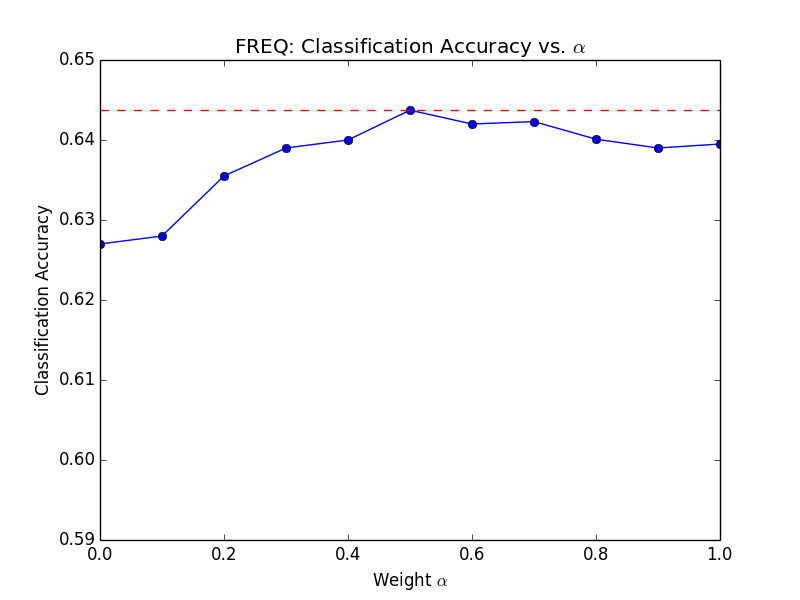
\includegraphics[width=3.2in]{ensemble_freq.png}
  \caption{Classification accuracy while varying $\alpha$.}
  \label{ensemble_freq}
\end{figure}

As expected, the graph for \textsc{Freq} has a peak at $\alpha=0.5$, which was the optimal value discovered earlier. Compared to if it were nonexistent ($\alpha=0$), the optimal addition of the \textsc{Freq} model increases our test accuracy by about 0.016. We can compare this to a similar graph of a model that did not perform very well standalone, such as \textsc{Sent}, shown in Figure~\ref{ensemble_sent}.

\begin{figure}[h]
  \centering
    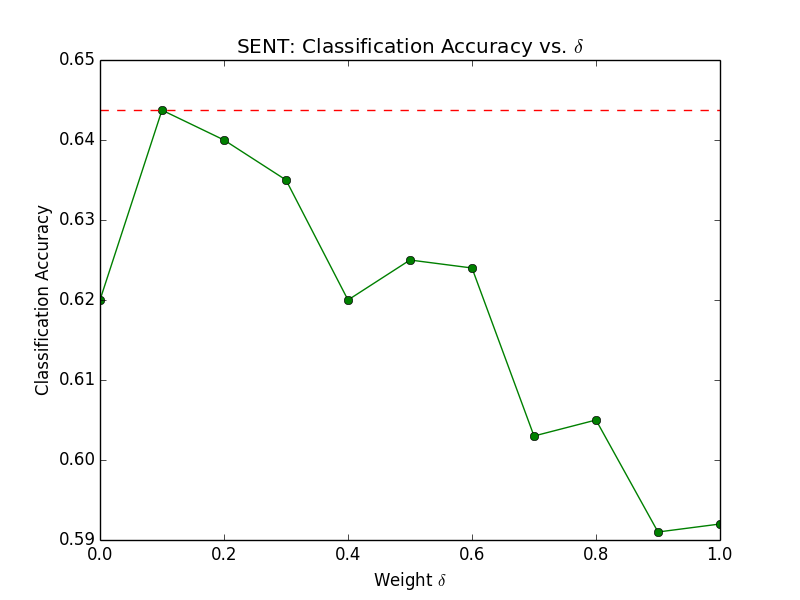
\includegraphics[width=3.2in]{ensemble_sent.png}
  \caption{Classification accuracy while varying $\delta$.}
  \label{ensemble_sent}
\end{figure}

Again, as expected, the graph for \textsc{Sent} has a peak at its optimal value $\alpha=0.1$. This time, however, we notice that the net contribution given by this model is larger at around 0.023. This is interesting when considering the fact that \textsc{Sent} was one of the poorer performing standalone models. This possibly suggests that sentiment analysis -- a very different approach to topic classification compared to those offered by standard word representations -- provides more new information that complements what has already been parsed, yielding better accuracy. Thus, in the face of the vast complexity given by Twitter content and language, our results suggest that an ensemble model which tries to capture a wide variety of features using different models may be an effective approach.

Building off the idea that different models identify different features, it is possible that different models may do better at classifying different topics. Thus, future work on this ensemble model could implement a weighting scheme that varies based on which topics are under consideration, allowing for a more fine-tune classification.

\section{Conclusion}

Our project explored many different word representations for the Tweet data as well as tested each on a variety of models in order to determine which would yield the best test accuracies. Additionally, we used the key points from various work in the area previously determined, and applied them to our task of classifying Tweets without the use of the main hashtag. Overall, the logistic regression and neural network models produced the best results, with the TF-IDF vector representation seemingly capturing the most information. Sentiment analysis and incorporation as a signal seemed to initially not produce a positive result, but when combined with other models in predicting on test data, led to a better performance and classification of some Tweets. Relation extraction showed promise as an addition to word representations as well. Finally, our ensemble model successfully took particular positive aspects of each model and signal, and produced a better model that captured different aspects in the train data that could not be covered by just a single model.

% include your own bib file like this:
%\bibliographystyle{acl}
%\bibliography{acl2014}

\begin{thebibliography}{1}

\bibitem{1} [1] K. Lee, D. Palsetia, R. Narayanan, M. Patwary, A. Agrawal, A. Choudhary. Twitter Trending Topic Classification. IEEE, 2011.

\bibitem{2} [2] D. Ramage, S. Dumais, D. Liebling. Characterizing Microblogs with Topic Models. AAAI, 2010.

\bibitem{3} [3] J. Li, A. Ritter, C. Cardie, and E. Hovy. Major Life Event Extraction from Twitter Based on Congratulations/Condolences Speech Acts. EMNLP, 2014.

\bibitem{4} [4] J. Pennington, R. Socher, C. Manning. GloVe: Global Vectors for Word Representation. EMNLP, 2014.

\bibitem{5} [5] Open Information Extraction System, v4.0. University of Washington. Accessed 6/1/2015word  at https://github.com/knowitall/openie.

\end{thebibliography}

\end{document}
